\chapter{\MakeUppercase{Resultados numéricos}}
%\chapter{Resultados numéricos}
\thispagestyle{fancy}
El algoritmo  mostrado en la Figura \ref{eqn:algoritmo}   es implementado con el software FreeFEM++  \cite{MR3043640} que permite escribir la formulación variacional de los problemas que definen la concentración de nutrientes, la presión intracelular, la extensión de la velocidad y evolución de la función conjunto de nivel.
\section{Aproximación de un problema elíptico en un dominio circular}
En primer lugar analizamos la convergencia numérica de la solución del problema test
\begin{equation}
	-\Delta u+ u =f \text{ en } \Omega\quad
	u=\kappa \text{ en } \partial \Omega
	\label{eqn:problematest1}
\end{equation}
que tiene solución exacta $u_{ex}=\dfrac{1}{R^3}(x^2+y^2)$ cuando $\Omega=\{(x,y):x^2+y^2<R^2\}$. $\kappa(x,y)=\dfrac{1}{R}$ y $f = \dfrac{1}{R^3}(x^2+y^2-4)$.

Definimos $\phi=\sqrt{x^2+y^2}-R$ y elegimos como dominio fijo $\mathcal{O}=]-8,8[\times ]-8,8[$, el cual es discretizado de manera uniforme con $n=8(2^i)$ triángulos en la dirección horizontal y vertical para $i=2,3,4,5$

Las medidas del error son las siguientes: 
\[
\epsilon_{L^2}=\dfrac{\|u_h-u_{ex}\|_{0,\Omega_h\setminus\Omega_h^\Gamma}}{\|u_{ex}\|_{0,\Omega_h\setminus\Omega_h^\Gamma}}
\]
\[
\epsilon_{H^1}=\dfrac{|u_h-u_{ex}|_{1,\Omega_h\setminus\Omega_h^\Gamma}}{|u_{ex}|_{1,\Omega_h\setminus\Omega_h^\Gamma}}
\]
%\begin{defi}
%	Sea $p_n$ una sucesión tal que $p_n\to p$ y que $p_n \neq p$ para todo $n$. Si
%	\[
%	\lim_{n\to\infty} \frac{|p_{n+1}-p|}{|p_n-p|^\alpha}=\lambda
%	\]
%	entonces la sucesión converge a $p$ con orden $\alpha$ y constante de error asintótica $\lambda$.
%\end{defi}
%Para estimar el orden de convergencia de los métodos desarrollados, haremos la aproximación
%\[
%\frac{|p_{n+1}-p|}{|p_n-p|^\alpha}\approx \lambda \implies
%\log|p_{n+1}-p|\approx \alpha \log|p_n-p|  +  \log\log\lambda 
%\]
%por lo que una gráfica log-log puede ayudar a visualizar el orden de convergencia mediante la pendiente de la recta de los datos observados.

Si asumimos que $
\|u_h-u_{ex}\|\approx C  \|u_{ex}\|h^{\alpha}$ para algún $C>0$, entonces una gráfica log-log puede ayudar a visualizar un valor aproximado para $\alpha$ mediante la pendiente de la recta ajustada a los datos obtenidos, la cual será indicada en cada gráfica.

En las Figuras \ref{fig:convergenciaphifemdual1}, \ref{fig:convergenciaphifemdual2}, \ref{fig:convergenciaphifemdual3} se muestra la variación de  $\epsilon_{L^2}$ y $\epsilon_{H^1}$ respecto a $h$ cuando $k=1$, $k=2$ y $k=3$ respectivamente y haciendo variar $l=k,k+1,k+2$. En todos los casos el orden de convergencia $\alpha$ estimado es $k+1$ en la norma de $L^2$ y $k$ para la seminorma de $H^1$, es decir:
\[
\|u_h-u_{ex}\|_{0,\Omega_h\setminus\Omega_h^\Gamma}
\approx C  \|u_{ex}\|^{k+1}_{0,\Omega_h\setminus\Omega_h^\Gamma}
\]
\[
|u_h-u_{ex}|_{1,\Omega_h\setminus\Omega_h^\Gamma}
\approx C  |u_{ex}|^{k}_{1,\Omega_h\setminus\Omega_h^\Gamma}
\]

\begin{figure}[H]
	\centering
	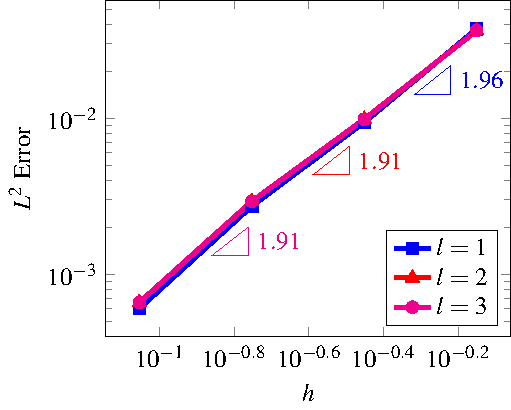
\includegraphics[width=0.4\linewidth]{img/convergenciaphifemdual1L2}\quad
	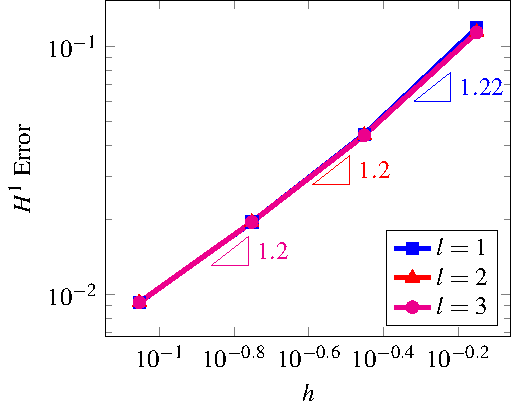
\includegraphics[width=0.4\linewidth]{img/convergenciaphifemdual1H1}
	\caption{Estimación del orden de convergencia  para la solución del problema mostrado en la ecuación \ref{eqn:problematest1} considerando $u_h\in V_h^{(1)}$,  y $\phi_h$ de tipo $\mathbb{ P}_l$. }
	\label{fig:convergenciaphifemdual1}
\end{figure}
\begin{figure}[H]
	\centering
	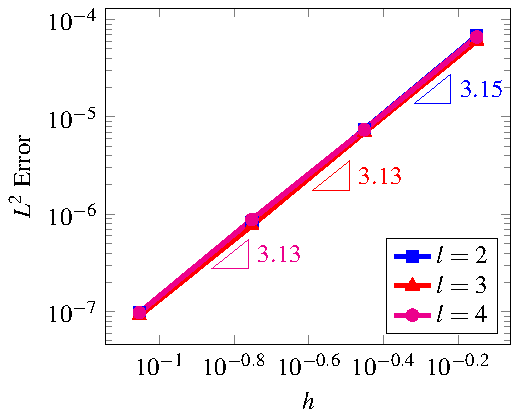
\includegraphics[width=0.4\linewidth]{img/convergenciaphifemdual2L2}\quad
	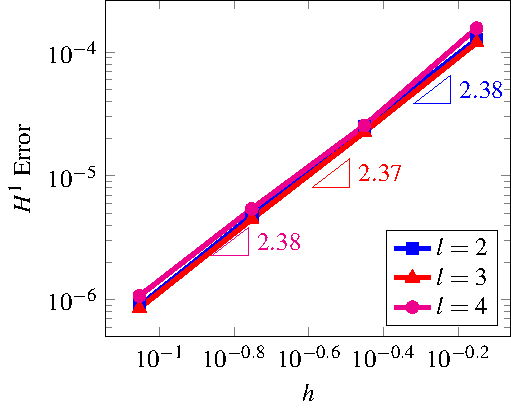
\includegraphics[width=0.4\linewidth]{img/convergenciaphifemdual2H1}
	\caption{Estimación del orden de convergencia  para la solución de la ecuación \ref{eqn:problematest1} considerando $u_h\in V_h^{(2)}$,  y $\phi_h$ de tipo $\mathbb{ P}_l$. }
	\label{fig:convergenciaphifemdual2}
\end{figure}

\begin{figure}[H]
	\centering
	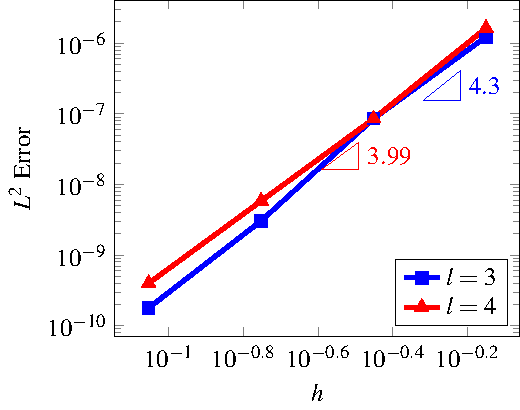
\includegraphics[width=0.4\linewidth]{img/convergenciaphifemdual3L2}\quad
	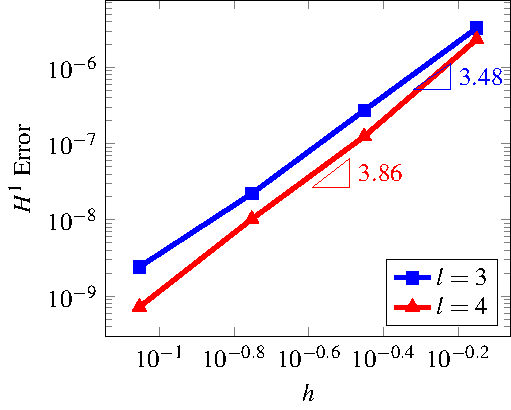
\includegraphics[width=0.4\linewidth]{img/convergenciaphifemdual3H1}
	\caption{Estimación del orden de convergencia  para la solución de la ecuación \ref{eqn:problematest1} considerando $u_h\in V_h^{(3)}$,  y $\phi_h$ de tipo $\mathbb{ P}_l$. }
	\label{fig:convergenciaphifemdual3}
\end{figure}
\section{Aproximación de la curvatura para el caso de un tumor con frontera circular}
Si consideramos que la curvatura de $\Gamma_h$ puede aproximarse por la ecuación \ref{eqn:curvaturaaproximacion} entonces el orden de convergencia estimado es $k+1$ en la norma de $L^2$ y $k$ para la seminorma de $H^1$, tal como se aprecia en la Figura  \ref{fig:convergenciaphifemdualcurvatura}.

\begin{figure}[H]
	\centering
	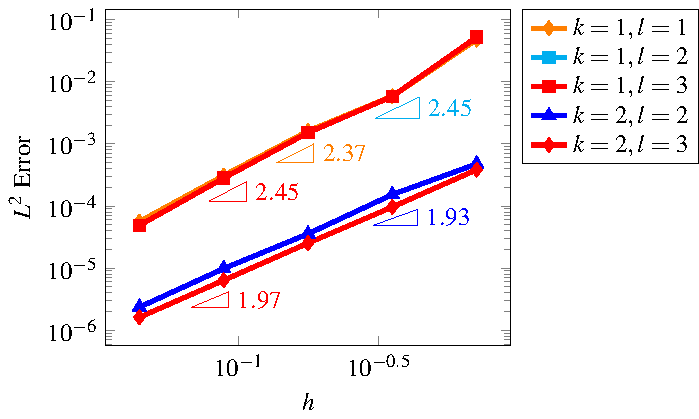
\includegraphics[width=0.6\linewidth]{img/convergenciaphifemdualcurvaturaL2}\quad
	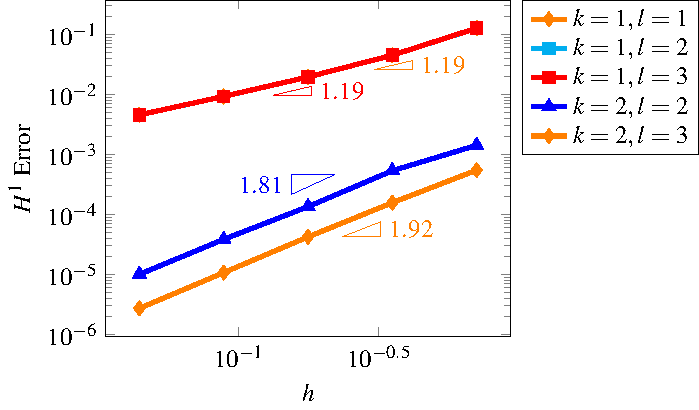
\includegraphics[width=0.6\linewidth]{img/convergenciaphifemdualcurvaturaH1}	
	\caption{Estimación del orden de convergencia  para la solución del problema \ref{eqn:curvaturaaproximacion} considerando $u_h\in V_h^{(k)}$,  y $\phi_h$ consta de elementos de tipo $\mathbb{ P}_l$.}
	\label{fig:convergenciaphifemdualcurvatura}
\end{figure}
\comentario{
	Para el caso del cálculo de la presión intracelular el problema \ref{eqn:phifemdual} se escribe como
	\begin{equation}
		\begin{aligned}
			\int_{\Omega_h}\nabla w \cdot \nabla v
			- \int_{\partial \Omega_h} \frac{\partial w}{\partial n}  v
			+ \frac{\gamma}{h^2}  \int_{\Omega_h^\Gamma} (w-\frac{1}{h}\phi_h p) (v-\frac{1}{h}\phi_h q)
			+G_h(w,v)+J_h^{lhs}(w,v)
			=\\
			\frac{\gamma}{h^2}  \int_{\Omega_h^\Gamma} \kappa_h (v-\frac{1}{h}\phi_h q)+J_h^{rhs}(v)
		\end{aligned}
	\end{equation}
	Es posible escribir el término $ \int_{\Omega_h^\Gamma} \kappa_h (v-\frac{1}{h}\phi_h q)$ como
	\[
	\int_{\Omega_h^\Gamma} \nabla\cdot\left(\frac{\nabla\phi_h}{|\nabla\phi_h|}\right) (v-\frac{1}{h}\phi_h q)= \int_{\partial\Omega_h^\Gamma} (v-\frac{1}{h}\phi_h q) \left(\frac{\nabla\phi_h}{|\nabla\phi_h|}\right)\cdot n
	- \int_{\Omega_h^\Gamma} \left(\frac{\nabla\phi_h}{|\nabla\phi_h|}\right) \cdot \nabla(v-\frac{1}{h}\phi_h q)
	\]
	Este cambio solo afecta al lado derecha de la ecuación así que el problema sigue teniendo solución única.
	
	
	En la Figura \ref{fig:convergenciacurvaturacirculo} se muestra el error cometido sobre la frontera $\Gamma_h$ cuando aproximamos la curvatura por $K_h$ para el caso de las curvas polares $r=4$ y $r=2.1 + 0.5\cos(2t)$ en un dominio global $\mathcal{O}=\left]-3,3\right[^2$. La curvatura para una curva polar $r=f(\theta)$ está dada por
	\[
	\kappa =\frac{2(f'(\theta))^2+(f(\theta))^2-f(\theta)f''(\theta)}{
		\left[
		(f'(\theta))^2+(f(\theta))^2
		\right]^{3/2}
	}
	\]
	y el error cometido en la aproximación esta definido por
	\[
	\epsilon_h =\|\kappa - K_h\|_{L^2(\Gamma_h)}
	\]
	así hemos encontrado una extensión suave de la curvatura definida sobre el dominio banda $\Omega_h$.
}
\section{Extensión de la velocidad definida sobre una interfase circular}
Consideremos el problema de interfase circular propuesto en \cite{utz2018high}: el dominio fijo es $\mathcal{O}=\left<-2,2\right>^2 \setminus [-\frac{1}{2},\frac{1}{2}]^2$ y la función conjunto de nivel es $\phi(x,y)=\sqrt{x^2+y^2}-1$ de manera que la interfase $\Gamma$ esta definida por $\left\{(x,y):\phi(x,y)=0\right\}$. Consideramos $u_0:\Gamma \to\mathbb{R}$ tal que 
\[
u_0(x,y)=1-x^2+y
\]
Como la rectas que contienen al origen, con ángulo de inclinación $\theta$ son normales a la interfase entonces la extensión $u:\mathcal{O}\to\mathbb{R}$ debe satisfacer que
\[
\begin{aligned}
	u(x,y) &= u_0(\cos \theta, \sen \theta)=1-\cos^2\theta  +\sen\theta \\
	&=1-\frac{x^2}{x^2+y^2}+\frac{y}{\sqrt{x^2+y^2}}\\
	&=y\left(\frac{y+\sqrt{x^2+y^2}}{\sqrt{x^2+y^2}}
	\right)
\end{aligned}
\]
Para estimar el orden de convergencia de la solución del problema \ref{eqn:problemaextension} se utilizan $2n^2$ elementos tipo $\mathbb{P}_k$, con $n=8\cdot 2^i$ para $i=2,3,4,5$ y $h=4\sqrt{2}/n$, los resultados se muestran en la Figura \ref{fig:convergenciaextension} considerando $k=1$, $k=2$, $k=3$. Así el orden de convergencia estimado en la norma $L^2$ es $k+1$ y en la norma $H^1$ es $k$.
\begin{figure}[H]
	\centering
	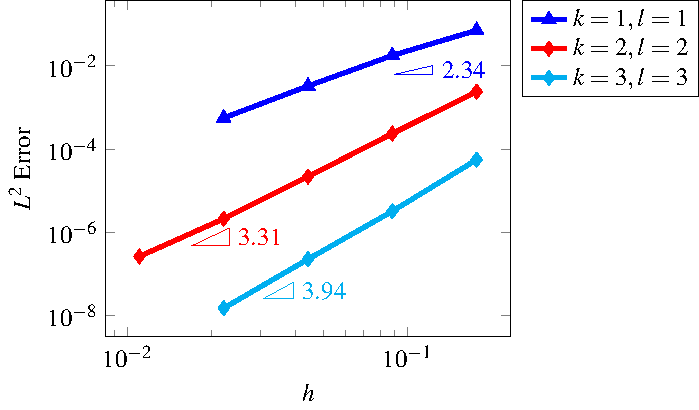
\includegraphics[width=0.6\linewidth]{img/convergenciaextensionL2}\quad
	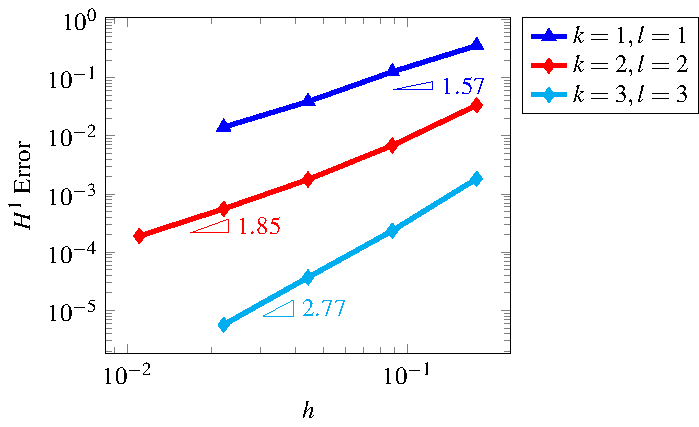
\includegraphics[width=0.6\linewidth]{img/convergenciaextensionH1}	
	\caption{Estimación del orden de convergencia  para la solución del problema \ref{eqn:problematest1} considerando $u_h\in V_h^{(k)}$, y $\phi_h$  de tipo $\mathbb{ P}_l$.}
	\label{fig:convergenciaextension}
\end{figure}
A continuación se calcula la extensión de la velocidad considerando elementos $\mathbb{P}_2$ triangulares $h=0.176777$ y  $n=32$,  sobre un mallado uniforme del dominio fijo $\mathcal{O}$. Como se observa en la Figura \ref{fig:extensioncurvas} las curvas de nivel de la extensión de la velocidad son ortogonales a la interfase circular, de igual modo en la Figura \ref{fig:extensionerror} se muestra como el error $u-u_h$ se propaga a través de las curvas de nivel de la extensión de la velocidad.
\begin{figure}[H]
	\centering
	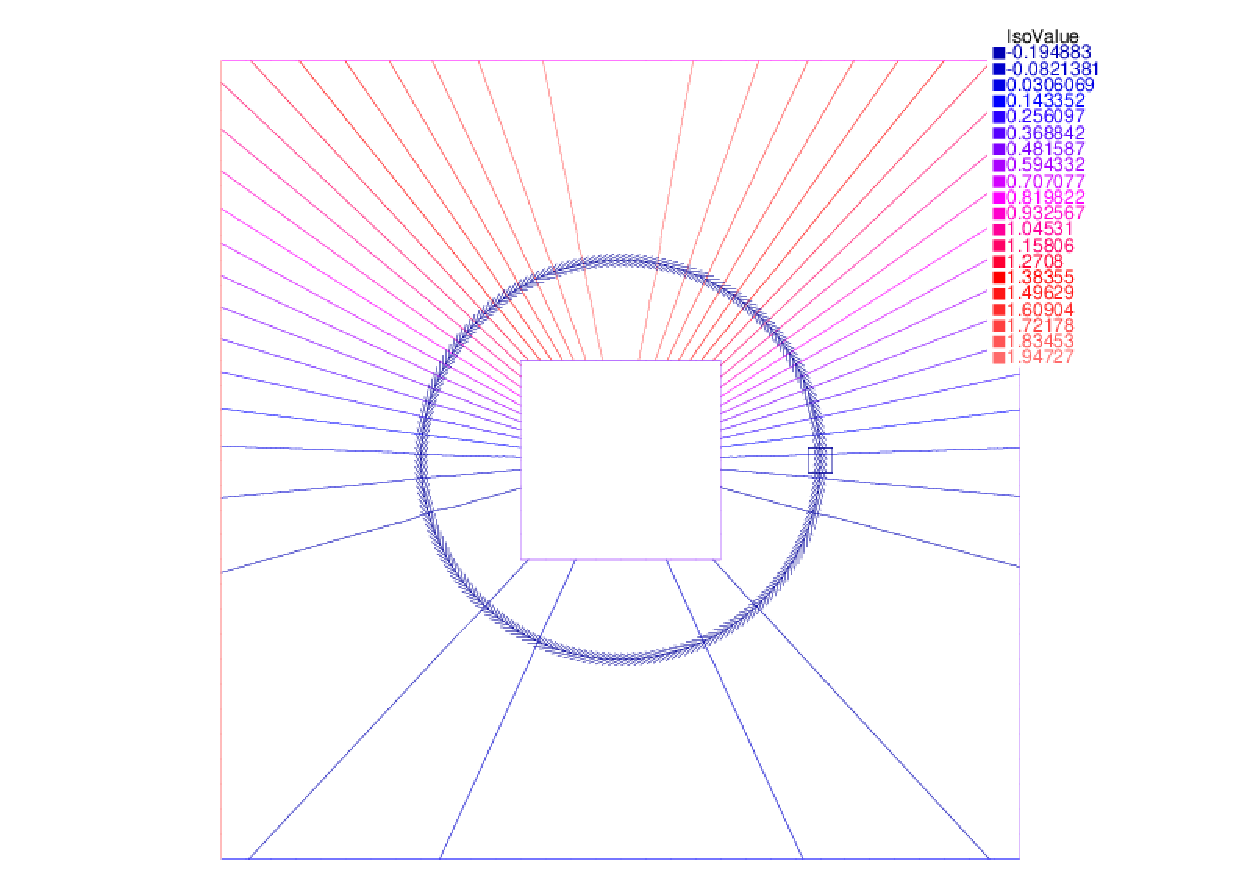
\includegraphics[width=0.7\linewidth]{img/extensioncurvas}	
	\caption{Curvas de nivel para la extensión de la velocidad en el caso de un interfase circular.}
	\label{fig:extensioncurvas}
\end{figure}
\begin{figure}[H]
	\centering
	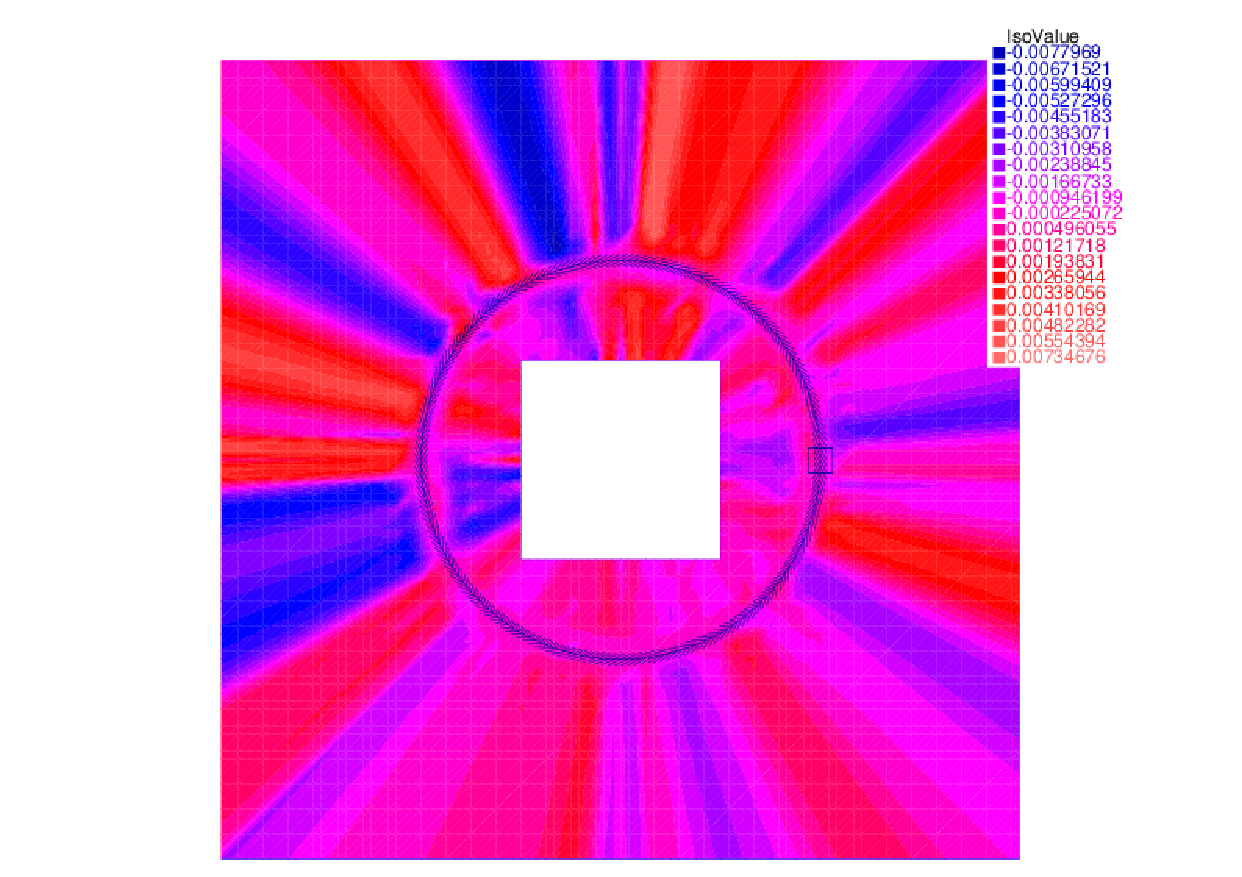
\includegraphics[width=0.7\linewidth]{img/extensionerror}
	\caption{Error de la aproximación de la extensión: $u-u_h$ para $k=l=2$ (elementos $\mathbb{ P}_2$)}
	\label{fig:extensionerror}
\end{figure}
\section{Extensión de la velocidad definida sobre una interfase no circular}
Consideremos la función conjunto de nivel $\phi(x,y)=x+x|y|$ de modo que la interfase $\Gamma$ corresponde con la recta vertical $x=0$, y tenemos $u_0:\Gamma \to\mathbb{R}$ una función que deseamos extender a una función $u:\Omega \to\mathbb{R}$ tal que $\Gamma\subset\Omega$ y $\Gamma \subset \Omega$. Para ello aplicamos el método de curvas características:
\[
\partial_x\phi(x,y) = 1+|y|, \text{si }x,y\in\mathbb{R}
\]
\[
\partial_y\phi(x,y) = \begin{cases}
	x,& \text{si }x\in\mathbb{R},y>0\\
	-x,& \text{si }x\in\mathbb{R},y<0\\
	0,& \text{si }x=0,y=0
\end{cases}
\]

luego una curva característica $\alpha$ está definida por la ecuaciones
\[
x'(t)=1+|y(t)|,\quad y'(t)=x
\]
\begin{figure}[H]
	\centering
	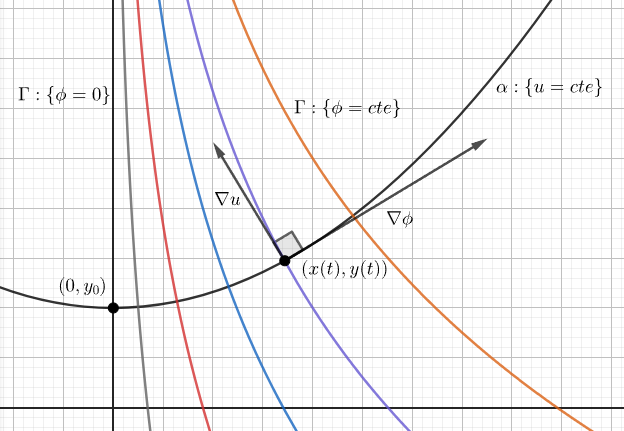
\includegraphics[width=0.7\linewidth]{img/extension}	
	\caption{Curvas características para la extensión de la velocidad cuando la interfase coincide con el eje $y$.}
	\label{fig:extensionnocircular}
\end{figure}
Si $y_0>0$ entonces $y(t)>0$, luego
\[
\frac{dy}{dt}=\frac{dy}{dx}\frac{dx}{dt}=\frac{dy}{dx}(1+y)=x
\]
integrando tenemos que
\[
2y+y^2 = x^2 + C
\]
y por la condición inicial $y(0)=y_0$, $x(0)=0$
\[
2y+y^2 = x^2 + 2y_0+y_0^2
\]
de donde 
\[
y_0 = \sqrt{(1+y)^2-x^2}-1
\]
de igual manera para $y_0<0$
\[
y_0 = 1-\sqrt{(1-y)^2-x^2}
\]
y como en la curva característica el valor de $u$ es constante, $u(x,y)=u(0,y_0)=u_0(y_0)$:
\[
u(x,y)=
\begin{cases}
	u_0(\sqrt{(1+y)^2-x^2}-1),&y>\sqrt{1+x^2}-1\\
	u_0(1-\sqrt{(1-y)^2-x^2}),&y<1-\sqrt{1+x^2}
\end{cases}
\]
Lo cual quiere decir que en la región donde $1+|y|<\sqrt{1+x^2}$ el problema está mal puesto y se tendrán resultados espurios al resolver la ecuación \ref{eqn:problemaSh}  con $\epsilon=0$, dicha perdida de regularidad se observa la Figura \ref{fig:extensionnocircular3d}; sin embargo considerando la Proposición \ref{prop:extension} con 
$\epsilon=10^{-2}$ garantizamos la existencia de solución única para el problema de extensión,  aunque ya no se tendrá la propagación de los valores de la interfase a través de las curvas de nivel tal como se observa en la Figura \ref{fig:extensionnocircularniveles}.

\begin{figure}[H]
	\centering	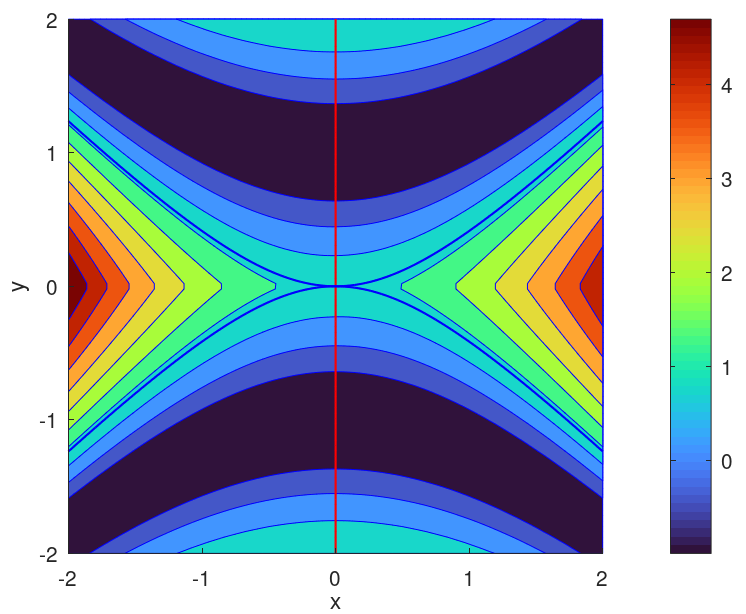
\includegraphics[width=0.6\linewidth]{img/extension1}	 \quad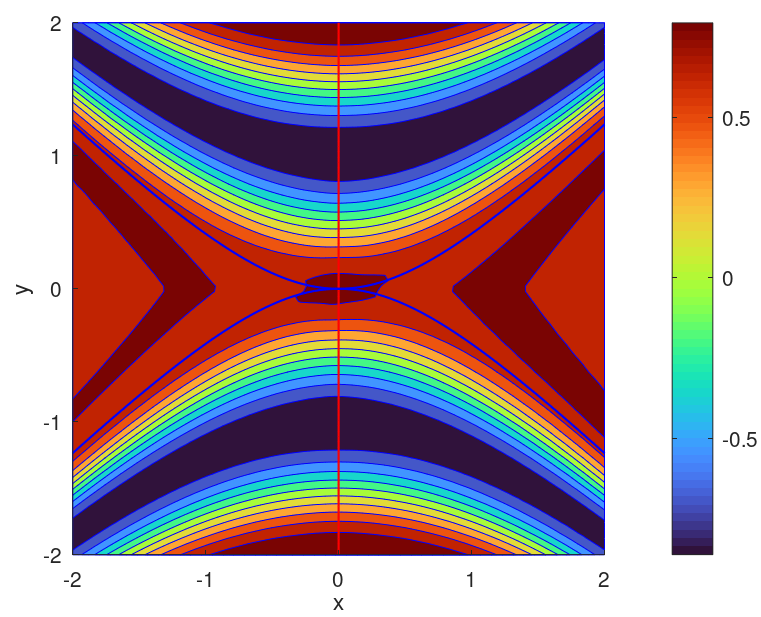
\includegraphics[width=0.6\linewidth]{img/extension2}
	\caption{Curvas de nivel para la extensión de la velocidad. Arriba: solución con $\epsilon=0$. Abajo:  solución con $\epsilon=10^{-2}$}	\label{fig:extensionnocircularniveles}
\end{figure}
\begin{figure}[H]
	\centering	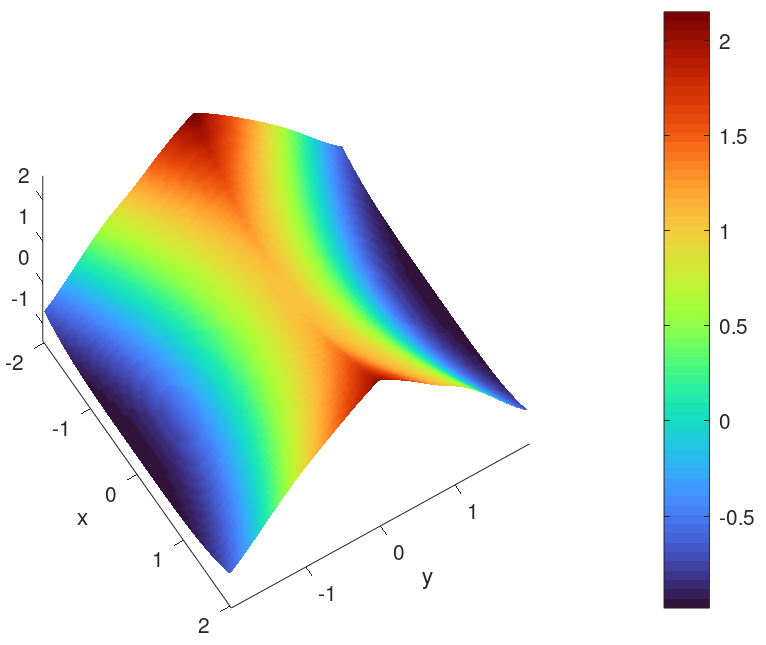
\includegraphics[width=0.6\linewidth]{img/extension3d1}	 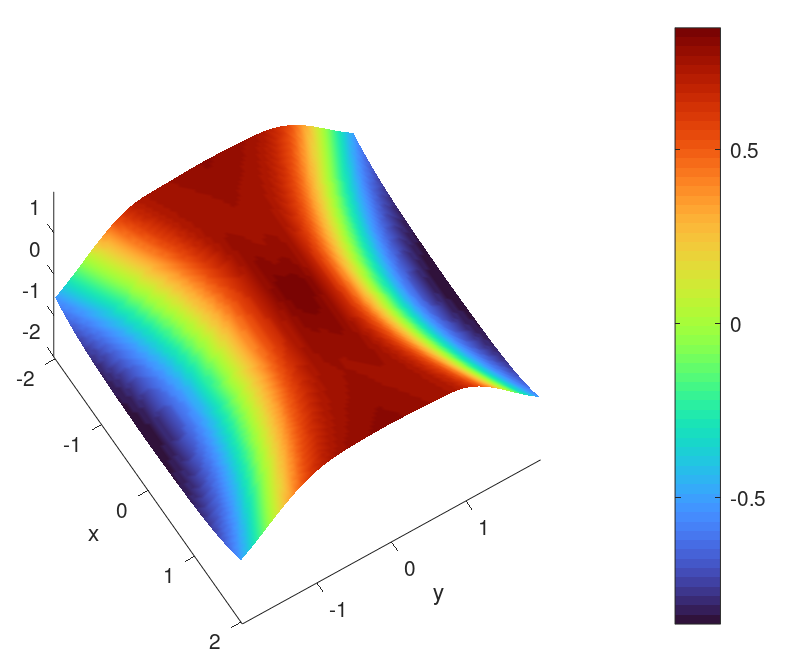
\includegraphics[width=0.6\linewidth]{img/extension3d2}
	\caption{Vista tridimensional de la extensión de la velocidad. Arriba: solución con $\epsilon=0$. Abajo:  solución con $\epsilon=10^{-2}$}	\label{fig:extensionnocircular3d}
\end{figure}
\section{Rotación de un dominio circular definido por una curva de nivel}
Consideremos $\phi_0(x,y)=\sqrt{(x-1)^2+y^2}-1$ y el campo de velocidades $(v_1,v_2)=(y,-x)$, con dominio fijo $\mathcal{O}=\left]-4,4\right[^2$. La interfase $\Gamma(t)$ esta definida por $\{(x,y):\phi(x,y,t)=0\}$ de modo que la ecuación de evolución de la función conjunto de nivel es
\[
\partial_t \phi + y\phi_x - x\phi_y=0
\]
Siguiendo el método de características, si $x(t),y(t)$ es tal que $\phi(x(t),y(t),t)=0$ entonces
\[
x'(t)=y(t)\quad y'(t)=-x(t)
\]
por lo tanto se se satisface el siguiente sistema desacoplado de EDO's
\begin{equation}
	\begin{aligned}
		x''(t)+x(t)=&0 \\
		y''(t)+y(t)=&0
	\end{aligned}
	\label{eqn:edo}
\end{equation}
además
\[
\frac{d}{dt}(x(t)^2+y(t)^2)=2(x'(t)x(t)+y'(t)y(t))=0
\]
lo cual indica que las curvas características son circunferencias centradas en el origen de radio $r=\sqrt{x_0^2+y_0^2}$.

Entonces la solución del sistema de EDO's (\ref{eqn:edo}) es \[
x(t)=x_0\cos t - y_0\sen t, \quad y(t)=x_0\sen t + y_0\cos t
\]

Al aplicar el método de aproximación por características de Galerkin (\ref{eqn:nuevophih}), considerando 2048 elementos triangulares $\mathbb{P}_2$ y $h=0.353553$ obtenemos la evolución de la interfase para $t=0, \frac{\pi}{2},\pi, \frac{3\pi}{2},2\pi$, como se muestra en la Figura \ref{fig:rotacion}.
\begin{figure}[H]
	\centering
	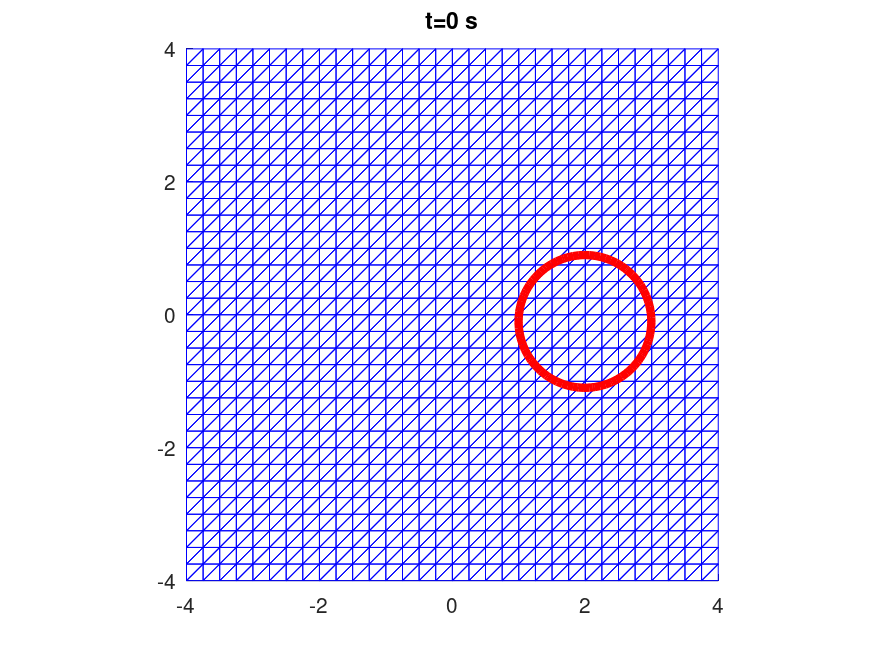
\includegraphics[width=0.4\linewidth]{img/rotacion1}
	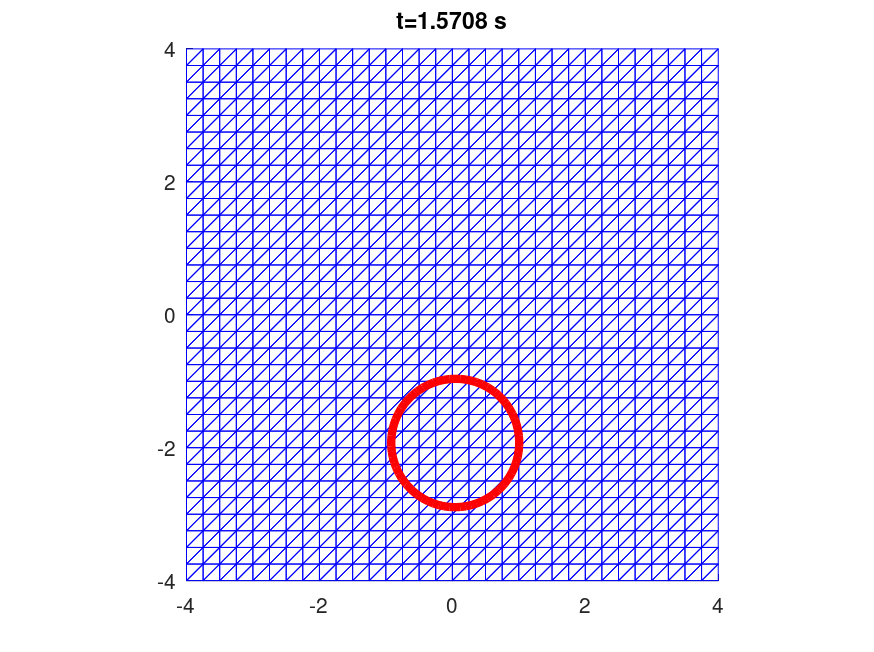
\includegraphics[width=0.4\linewidth]{img/rotacion2}
	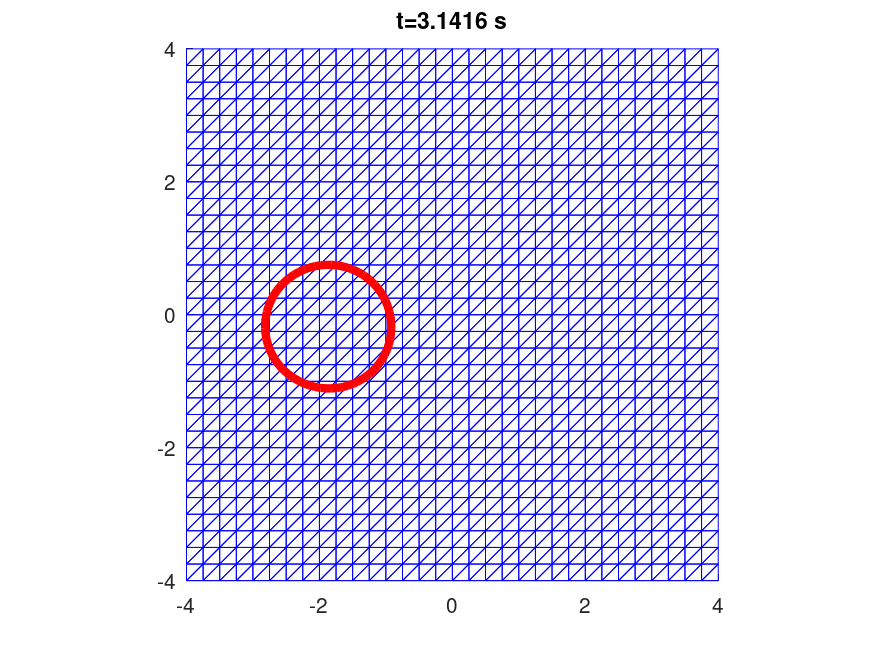
\includegraphics[width=0.4\linewidth]{img/rotacion3}
	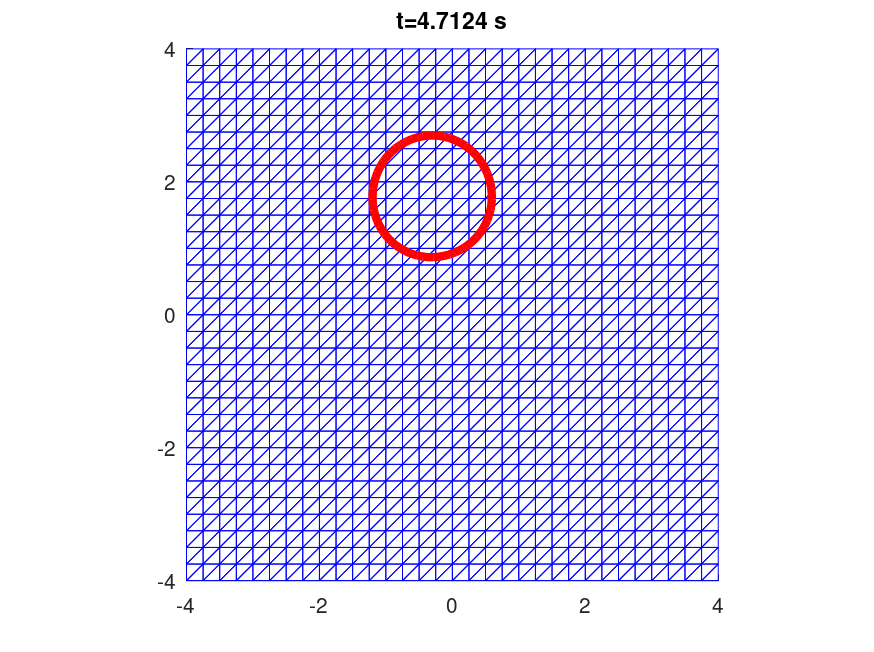
\includegraphics[width=0.4\linewidth]{img/rotacion4}
	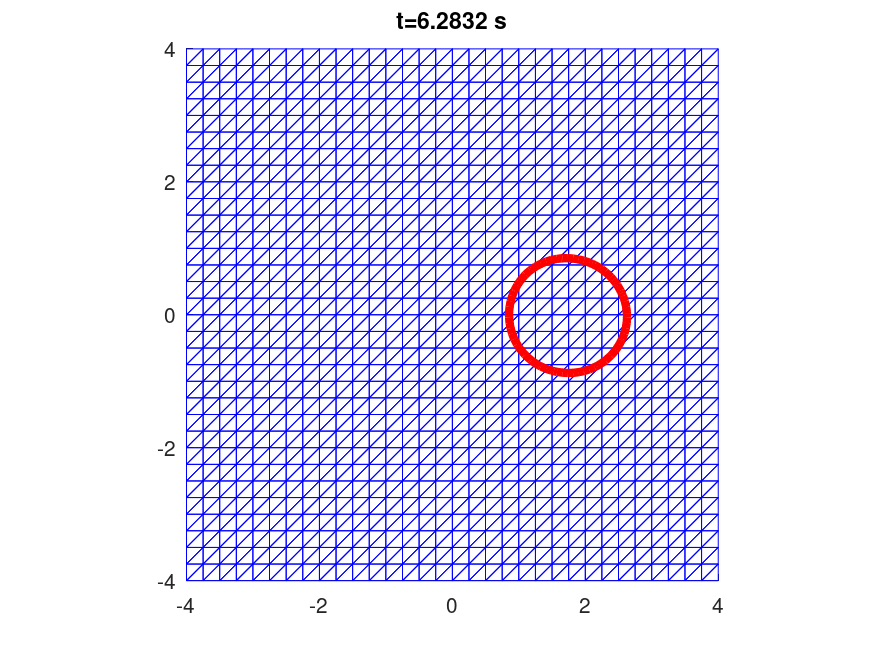
\includegraphics[width=0.4\linewidth]{img/rotacion5}
	\caption{Evolución de la interfase circular $\Gamma(t)$ si  $\Gamma(0):=\{(x,y):\phi_0(x,y)=0\}$}
	\label{fig:rotacion}
\end{figure}


\section{Solución exacta del crecimiento tumoral con simetría radial}
En este caso simulamos la evolución del crecimiento de un tumor con frontera inicial circular en etapa de baja vascularización y que por lo tanto se acerca a la solución estacionaria con radio $R_\infty$ dado por la ecuación \ref{eqn:radioestacionario}. Escogemos los parámetros 
$R(t=0)=4$, $A=1/2$, $G=20$, de modo que 
\[
2.8284\approx \sqrt{8}<R_\infty <4
\]
Los valores mostrados en el cuadro \ref{tabla:solucioncircular} son  calculados al resolver numéricamente la ecuación \ref{eqn:edoradiotumor} por medio del método de Adams predictor-corrector implementado por la librería LSODE parte de ODEPACK  \footnote{\url{https://computing.llnl.gov/projects/odepack}}  \cite{radhakrishnan1993description}. 
\begin{table}[H]
	\footnotesize
	\centering
	\caption{Velocidad de crecimiento en la frontera de un tumor con simetría circular de radio $R$.}
	\label{tabla:solucioncircular}
	\begin{tabular}{ccc}
		\toprule
		$t$&$V(t)$&$R(t)$ \\
		\midrule
		0  &-2.7295  & 4.0000 \\
		0.1000 & -1.7979 &  3.7771\\
		0.2000 & -1.1957 &  3.6295\\
		0.3000 & -0.8010 &  3.5310\\
		0.4000 & -0.5395 &  3.4649\\
		0.5000 & -0.3648 &  3.4203\\
		0.6000 & -0.2473 &  3.3900\\
		0.7000 & -0.1680 &  3.3695\\
		0.8000 & -0.1142 &  3.3556\\
		0.9000&  -0.0778 &  3.3461\\
		1.0000 & -0.0530 &  3.3397\\
		\bottomrule
	\end{tabular}
	
\end{table}
En las Figuras \ref{fig:crecimientoa05R04}-\ref{fig:crecimientoa05R02} se muestra el comportamiento del radio del tumor así como la velocidad en la frontera, y se observa que se estabilizan alrededor de la solución estacionaria asociada a $R_\infty$.
\begin{figure}[H]
	\centering
	\includegraphics[width=0.7\linewidth]{crecimientoa05R04}
	\caption{Solución numérica de la ecuación \ref{eqn:edoradiotumor} con los parámetros $R_0=4$, $A=0.5$, $G=20$.}
	\label{fig:crecimientoa05R04}
\end{figure}
\begin{figure}[H]
	\centering
	\includegraphics[width=0.7\linewidth]{crecimientoa05R02}
	\caption{Solución numérica de la ecuación \ref{eqn:edoradiotumor} con los parámetros $R_0=2$, $A=0.5$, $G=20$}
	\label{fig:crecimientoa05R02}
\end{figure}

En el caso que $A\geq 1$ y $G>0$ tenemos que
\[
-\frac{A}{2}<\frac{1}{w_0}-\frac{A}{2}<\frac{1-A}{2}\leq 0\implies V< 0
\]
por lo que $R$ es decreciente, y el tumor tiende a extinguirse como se aprecia en  la Figura \ref{fig:crecimientoa1dot5g20}.

\begin{figure}[H]
	\centering
	\includegraphics[width=0.7\linewidth]{crecimientoa1dot5G20}
	\caption{Solución numérica de la ecuación \ref{eqn:edoradiotumor} con los parámetros $A=1.5$, $G=20$}
	\label{fig:crecimientoa1dot5g20}
\end{figure}

\begin{figure}[H]
	\centering
	\includegraphics[width=0.7\linewidth]{crecimientoa0}
	\caption{Solución numérica de la ecuación \ref{eqn:edoradiotumor} con los parámetros $R_0=4$, $A=0.0$, $G=20$}
	\label{fig:crecimientoa0}
\end{figure}
\begin{figure}[H]
	\centering
	\includegraphics[width=0.7\linewidth]{crecimientoa-05G10}
	\caption{Solución numérica de la ecuación \ref{eqn:edoradiotumor} con los parámetros $R_0=2$, $A=-0.5$, $G=10$}
	\label{fig:crecimientoa-05G10}
\end{figure}
\section{Experimentos numéricos para el crecimiento de un tumor no circular} 
En las Figuras \ref{fig:evolucionnutrientesA}-\ref{fig:evolucionpresionA} los valores que identifican el régimen de baja vascularidad son $G=20$, $A=0.5$ y la frontera inicial del tumor está dada por la curva polar 
\begin{equation}
	r=2.1+0.5\cos(2\theta)
	\label{eqn:casoA}
\end{equation}
\begin{figure}[H]
	\centering
	\includegraphics[width=0.4\linewidth]{casoA/nutrientes0}
	\includegraphics[width=0.4\linewidth]{casoA/nutrientes400}
	\includegraphics[width=0.4\linewidth]{casoA/nutrientes800}
	\includegraphics[width=0.4\linewidth]{casoA/nutrientes1000}
	\caption{Evolución de la concentración de nutrientes al interior del tumor de frontera inicial dada por la ecuación \ref{eqn:casoA}, $A=0.5$, $G=20$}
	\label{fig:evolucionnutrientesA}
\end{figure}
\begin{figure}[H]
	\centering
	\includegraphics[width=0.4\linewidth]{casoA/presion0}
	\includegraphics[width=0.4\linewidth]{casoA/presion400}
	\includegraphics[width=0.4\linewidth]{casoA/presion800}
	\includegraphics[width=0.4\linewidth]{casoA/presion1000}
	\caption{Evolución de la presión al interior del tumor de frontera inicial dada por la ecuación \ref{eqn:casoA}, $A=0.5$, $G=20$}
	\label{fig:evolucionpresionA}
\end{figure}
En las Figuras \ref{fig:evolucionnutrientesB}-\ref{fig:evolucionpresionB} los valores que identifican el régimen de alta vascularización son $G=-5$, $A=0.8$ y la frontera inicial del tumor está dada por la curva polar 
\begin{equation}
	r= 2 + 0.24\cos(2\theta) + 0.2\sin(2\theta) + 0.12\cos(3\theta) + 0.1\sen(3\theta)+0.08\cos(5\theta)+ 0.14\sen(6\theta)
	\label{eqn:casoB}
\end{equation}
\begin{figure}[H]
	\centering
	\includegraphics[width=0.4\linewidth]{casoB/nutrientes0}
	\includegraphics[width=0.4\linewidth]{casoB/nutrientes400}
	\includegraphics[width=0.4\linewidth]{casoB/nutrientes800}
	\includegraphics[width=0.4\linewidth]{casoB/nutrientes1000}
	\caption{Evolución de la concentración de nutrientes al interior del tumor de frontera inicial dada por la ecuación \ref{eqn:casoB}, $A=0.8$, $G=-5$}
	\label{fig:evolucionnutrientesB}
\end{figure}
\begin{figure}[H]
	\centering
	\includegraphics[width=0.4\linewidth]{casoB/presion0}
	\includegraphics[width=0.4\linewidth]{casoB/presion400}
	\includegraphics[width=0.4\linewidth]{casoB/presion800}
	\includegraphics[width=0.4\linewidth]{casoB/presion1000}
	\caption{Evolución de la presión al interior del tumor de frontera inicial dada por la ecuación \ref{eqn:casoB}, $A=0.8$, $G=-5$}
	\label{fig:evolucionpresionB}
\end{figure}
En las Figuras \ref{fig:evolucionnutrientesC}-\ref{fig:evolucionpresionC} se observa el decrecimiento de un tumor con régimen de alta vascularización identificado por $G=-5$, $A=0.2$. y la frontera inicial del tumor está dada por la curva polar 
\begin{equation}
	r = 2 + 0.24\cos(2\theta) + 0.2\sen(2\theta) + 0.12\cos(3\theta)  + 0.1 \sen(3\theta)
	\label{eqn:casoC}
\end{equation}
\begin{figure}[H]
	\centering
	\includegraphics[width=0.4\linewidth]{casoC/nutrientes0}
	\includegraphics[width=0.4\linewidth]{casoC/nutrientes400}
	\includegraphics[width=0.4\linewidth]{casoC/nutrientes800}
	\includegraphics[width=0.4\linewidth]{casoC/nutrientes1000}
	\caption{Evolución de la concentración de nutrientes al interior del tumor de frontera inicial dada por la ecuación \ref{eqn:casoC}, $A=0.2$, $G=-5$} 	
	\label{fig:evolucionnutrientesC}
\end{figure}
\begin{figure}[H]
	\centering
	\includegraphics[width=0.4\linewidth]{casoC/presion0}
	\includegraphics[width=0.4\linewidth]{casoC/presion400}
	\includegraphics[width=0.4\linewidth]{casoC/presion800}
	\includegraphics[width=0.4\linewidth]{casoC/presion1000}
	\caption{Evolución de la presión al interior del tumor de frontera inicial dada por la ecuación \ref{eqn:casoC}, $A=0.2$, $G=-5$}	
	\label{fig:evolucionpresionC}
\end{figure}
En las Figuras \ref{fig:evolucionnutrientesD}-\ref{fig:evolucionpresionD} se observa el crecimiento de un tumor con régimen de alta vascularización identificado por $G=-5$, $A=0.8$. y la frontera inicial del tumor está dada por la curva polar mostrada en la ecuación \ref{eqn:casoC}.
\begin{figure}[H]
	\centering
	\includegraphics[width=0.4\linewidth]{casoD/nutrientes0}
	\includegraphics[width=0.4\linewidth]{casoD/nutrientes500}
	\includegraphics[width=0.4\linewidth]{casoD/nutrientes1000}
	\includegraphics[width=0.4\linewidth]{casoD/nutrientes1500}
	\caption{Evolución de la concentración de nutrientes al interior del tumor de frontera inicial dada por la ecuación \ref{eqn:casoC}, $A=0.8$, $G=-5$} 	
	\label{fig:evolucionnutrientesD}
\end{figure}
\begin{figure}[H]
	\centering
	\includegraphics[width=0.4\linewidth]{casoD/presion0}
	\includegraphics[width=0.4\linewidth]{casoD/presion500}
	\includegraphics[width=0.4\linewidth]{casoD/presion1000}
	\includegraphics[width=0.4\linewidth]{casoD/presion1500}
	\caption{Evolución de la presión al interior del tumor de frontera inicial dada por la ecuación \ref{eqn:casoC}, $A=0.8$, $G=-5$}	
	\label{fig:evolucionpresionD}
\end{figure}
\comentario{
	\section{Convergencia numérica del problema de Poisson}
	Para las experiencias numéricas se considera resolver el problema $-\Delta u +u = f \text{ en }\Omega, u=g\text{ en }\partial\Omega$ con
	$\Omega = \{x^2+y^2\leq 1/16 \}$ contenido en un dominio fijo  $\mathcal{O}=(-0.5,0.5)^2$. La solución exacta es $u_{ex}=\sen(x)\exp(y)$ si $f=u_{ex}$, y  $g=u_{ex}$.
	
	
	
	\begin{figure}[H]	
		\centering
		\includegraphics[width=0.4\linewidth]{convergenciafem.pdf}
		\includegraphics[width=0.4\linewidth]{problemaEDP}
		
	\end{figure}
	
	\begin{figure}[H]
		\centering	\includegraphics[width=0.4\linewidth]{convergenciaphifemduala}\hfil
		\includegraphics[width=0.4\linewidth]{convergenciaphifemdualb}\\
		\includegraphics[width=0.4\linewidth]{convergenciaphifemdualc}
		\caption{Convergencia de la solución numérico del problema \ref{eqn:phifemdual}. Izquierda error relativo $L^2$}
		\label{fig:convergenciaphifemduala}
	\end{figure}
	\section{Esquema de estabilización de la curvatura}
	\begin{figure}[H]
		\centering	
		\includegraphics{convergenciacurvaturacirculo}
		\caption{Error en la aproximación de la curvatura de una curva polar $r=f(\theta)$}
		\label{fig:convergenciacurvaturacirculo}
	\end{figure}
	
	\begin{figure}[H]
		\centering
		\includegraphics[width=0.7\linewidth]{curvaturaperturbacion}
		\caption{$\Omega_h$ y extensión de la curvatura $K_h$ para $r=2.1 + 0.5\cos(2\theta)$.}
		\label{fig:curvaturaperturbacion}
	\end{figure}
	\begin{figure}[H]
		\centering
		\includegraphics[width=0.7\linewidth]{curvaturacirculo}
		\caption{$\Omega_h$ y extensión de la curvatura $K_h$ para $r=2.1$.		
		}
		\label{fig:curvaturacirculo}
	\end{figure}
	
	
	\subsection{Convergencia, caso frontera libre circular}
	Para las experiencias numéricas se elige una función conjunto de nivel $\phi_0=x^2+y^2-4$ definida en primer caso sobre $D_1=(-4,4)^2$ y luego sobre $D_2=(-4,4)^2\setminus [-0.4,0.4]^2$,  de modo que en el segundo caso no se considera el origen pues la función distancia dirigida $\phi=\sqrt{x^2+y^2}-2$ no es diferenciable en el origen y el orden de convergencia se ve afectado. En la Figura \ref{fig:levelsetcircular} se muestra el orden de convergencia para valores de $h$ correspondiente a una triangulación uniforme con $n=8(2^i)$, subdivisiones para $i=0,1,\ldots, 6$.
	
	\begin{figure}[H]
		\includegraphics{reinicializacionradioconstantea.pdf}
		~%
		\includegraphics{reinicializacionradioconstanteb.pdf}
		%
		%
		\includegraphics{reinicializacionradioconstantec.pdf}
		~%
		\includegraphics{reinicializacionradioconstanted.pdf}
		\caption{Errores y orden de convergencia de la reinicialización de la función conjunto de nivel}
		\label{fig:levelsetcircular}
	\end{figure}
	
	
	\subsection{Convergencia, caso frontera libre de radio variable}
	Para las experiencias numéricas se elige una función conjunto de nivel \[
	\phi_0=x^2+y^2 - (2.1 + 0.5\cos(2\arctan(\frac{y}{x}))
	\] definida en un dominio banda $D$ tal que $\{\phi_0=0\}\subset D$ de modo que la reinicialización se realice solo en los elementos cercanos a la frontera libre. El dominio banda depende de la triangulación utilizada por lo tanto para comparar errores calculados en malla distintas, utilizaremos el error normalizado por unidad de área, $\dfrac{\epsilon_{SD}}{|D|}$. En la Figura \ref{fig:levelsetvariable} se muestra el orden de convergencia para valores de $h$ correspondiente a una triangulación uniforme con $n=8(2^i)$, subdivisiones para $i=1,\ldots, 6$.
	
	\begin{figure}[H]
		\includegraphics{reinicializacionradiovariablea.pdf}%
		\includegraphics{reinicializacionradiovariableb.pdf}
		\caption{Errores y orden de convergencia de la reinicialización de la función conjunto de nivel}
		\label{fig:levelsetvariable}
	\end{figure}
	
	\subsection{Convergencia, caso frontera con esquinas}
	Siguiendo a \citep{min2010reinitializing} se considera el caso de dos círculos de radio $r$ con centros $C_1=(-a,0)$, $C_2=(a,0)$, ($0<a<r$) tal que se interceptan en $V_1=(0,\sqrt{r^2-a^2})$, $V_2=(0,-\sqrt{r^2-a^2})$, de modo que la frontera libre este formada por la frontera de la unión de dichos círculos. La función distancia dirigida en este caso es
	\[
	\phi(x,y)=\begin{cases}
		-\min \left\{ d((x,y),V_i),i=1,2\right\} &,\text{ si } \frac{x+a}{d((x,y),V_1)}\geq \frac{a}{r} \text{ y }
		\frac{a-x}{d((x,y),V_2)}\geq \frac{a}{r},
		\\
		\min \left\{ d((x,y),C_i),i=1,2\right\}-r&
		,\text{ en otro caso.}
	\end{cases}
	\]
	Como función inicial tenemos 
	\[
	\phi^{0} = \phi \cdot \left[ (x-1)^2+ (y-1)^2 + 0.1\right]
	\]
	%\[
	%\phi^{0,b} = \phi \cdot \left[ 0.5 \sen(6\pi x)\sen (6\pi y) %+ 1\right]
	%\]
	\begin{figure}[H]
		\centering
		\includegraphics[width=0.7\linewidth]{lsconesquinasphi0amanchas}
		%	\includegraphics[width=0.7\linewidth]{lsconesquinasphi0bmanchas}
		\caption{Curvas de nivel para $\phi^{0}$}
		\label{fig:lsconesquinasphi0amanchas}
	\end{figure}
	
	\begin{figure}[H]
		\includegraphics{reinicializacionfronteraesquinaa.pdf}
		\includegraphics{reinicializacionfronteraesquinab.pdf}
		\includegraphics{reinicializacionfronteraesquinac.pdf}
		\includegraphics{reinicializacionfronteraesquinad.pdf}
		
		\caption{Errores y orden de convergencia de la reinicialización de la función conjunto de nivel en el caso de una frontera con esquinas o picos.}
		\label{fig:levelsetconesquinas}
	\end{figure}
}

\comentario{
	%%%%%%%%%%%% grafica la frontera libre %%%%%%%%%%%%%%%%%%
	figure;
	[xmesh,~,ymesh,~]=prepare_mesh(p,t);
	x=linspace(-2,2,100);
	y=linspace(-2,2,100);
	[X,Y]=meshgrid(x,y);
	[~,pdeData]=convert_pde_data(p,t,Sh,uh');
	PP=fftri2grid(X,Y,xmesh,ymesh,pdeData{1});
	hold on;
	PE=X;
	%contourf(X,Y,PP,"linewidth",2,"k.-");
	colormap ("turbo"); colorbar ();
	
	%contourf(X,Y,PP,"linewidth",0.5,"b");
	surf(X,Y,PP);
	shading interp;
	%contour(X,Y,PE,[0,0],"linewidth",1,"r-");
	%plot(x, sqrt(x.^2+1)-1,"linewidth",1,"b-",x,1-sqrt(x.^2+1),"linewidth",1,"b-");
	xlabel("x");
	ylabel("y");
	axis("equal");
	view([ 58.065,61.996])
	%title(["t=",num2str(step*i)," s"]);
	print(["extension1.png"])
	
	figure;
	
	[~,pdeData]=convert_pde_data(p,t,Sh,wh');
	PP=fftri2grid(X,Y,xmesh,ymesh,pdeData{1});hold on;
	colormap ("turbo"); colorbar ();
	
	%contourf(X,Y,PP,"linewidth",0.5,"b");
	surf(X,Y,PP);
	shading interp;
	
	%contour(X,Y,PE,[0,0],"linewidth",1,"r-");
	%plot(x, sqrt(x.^2+1)-1,"linewidth",1,"b-",x,1-sqrt(x.^2+1),"linewidth",1,"b-");
	xlabel("x");
	ylabel("y");
	axis("equal");
	%title(["t=",num2str(step*i)," s"]);
	view([ 58.065,61.996])
	print(["extension2.png"])
}